\setcounter{secnumdepth}{0}
\section*{Dodatek A: Instrukcja}\label{zajecia-dydaktyczne}
\addcontentsline{toc}{section}{\protect\numberline{}Dodatek A: Zajęcia dydaktyczne}

\subsection{Wejściówka}

Na samym początku zajęć odbędzie się wejściówka składająca się z pytań otwartych
i zamkniętych.
Przykładowe pytania, które mogą znaleźć się na wejściówce to:

\begin{enumerate}
    \item Podaj definicję dodawania i mnożenia w $\mathbb{F}_2$ bądź wypisz wynik tych
    działań dla wszystkich możliwych kombinacji elementów.
    \item Czym się różni słowo kodowe wygenerowane kodem systematycznym i niesystematycznym
    \item Ile błędnych symboli jest w stanie wykryć lub poprawić kod Reeda-Solomona
    \begin{enumerate}[label=\Alph*:]
        \item wykryć: $n-k$, poprawić: $n-k-1$
        \item wykryć: $n-k-1$, poprawić: $n-k-1$
        \item wykryć: $\lfloor \frac{n-k}{2} \rfloor$, poprawić: $\lfloor \frac{n-k}{2} \rfloor$
        \item wykryć: $n-k$, poprawić: $\lfloor \frac{n-k}{2} \rfloor$
    \end{enumerate}
    \item Podaj zaletę oraz wadę stosowania większej ilości poziomów w modulacjach PAM
    \item Czym się różni szerokość pasma od przepustowości?
    \item Opisz krótko czym jest NRZ (Non-Return-to-Zero)
    \item Czym jest przepływność łącza?
\end{enumerate}

\subsection{Narzędzia}

\subsubsection{Symulator - wybór technologii}
Do stworzenia symulatora wybrano język programowania Python i wykorzystano między innymi następujące gotowe rozwiązania:

\begin{enumerate}
    \item PyQt będzie biblioteką wykorzystywaną do stworzenia interfejsu graficznego użytkownika (GUI) dla symulatora. PyQt zapewnia szeroki zakres narzędzi do tworzenia rozbudowanych i przyjaznych użytkownikowi interfejsów, co jest szczególnie ważne w symulatorze dydaktycznym, gdzie interfejs musi być intuicyjny i nie stanowić niepotrzebnego wyzwania lub problemu dla biorących udział w zajęciach,
    \item NumPy jest najpopularniejszą biblioteką Python implementującą algorytmy matematyczne. Między innymi oferuje generatory liczb pseudolosowych o różnych rozkładach, co jest wymagane do prawidłowego generowania ramek ethernetowych i błędów,
    \item  Matplotlib to popularna biblioteka do tworzenia wykresów, przydatna przy tworzeniu wykresów sygnałów,
    \item SPICE (Simulation Program with Integrated Circuit Emphasis) jest powszechnie stosowanym narzędziem do symulacji obwodów elektronicznych. Jest to rozbudowany program, który umożliwia modelowanie i analizę zachowania obwodów złożonych, takich jak układy analogowe, cyfrowe czy mikroelektroniczne. W celu korzystania z tego narzędzia w środowisku Python dostępna jest biblioteka PySpice, będąca interfejsem umożliwiającym korzystanie ze SPICE,
\end{enumerate}

\subsubsection{Interfejs użytkownika}
Interfejs użytkownika został wykonany przy użyciu PyQt5 oraz Qt Designer. Qt Designer to graficzne narzędzie do projektowania interfejsów użytkownika w ramach frameworka Qt. Umożliwia łatwe tworzenie i dostosowywanie wyglądu aplikacji oraz następne jego wygenerowanie jako kodu w języku Python lub C++.

Interfejs składa się z kilku zakładek stworzonych, które umożliwiają przełączanie między częściami aplikacji bez utraty wyników dotychczasowej pracy. Każda zakładka przeznaczona jest do innego zadania laboratoryjnego i zawiera symulacje innych rozwiązań ethernetowych.

\begin{figure}[ht]
    \centering
    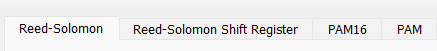
\includegraphics{images/zakladki.png}
    \caption{Zakładki symulatora}
    \label{fig:zakladki_image}
\end{figure}

Wykresy są tworzone przy pomocy biblioteki Matplotlib. Została dodatkowo stworzona klasa, która zawiera stworzone wykresy i może być użyta jako element graficznego interfejsu użytkownika, a więc dodana do niego.

\begin{figure}[ht]
    \centering
    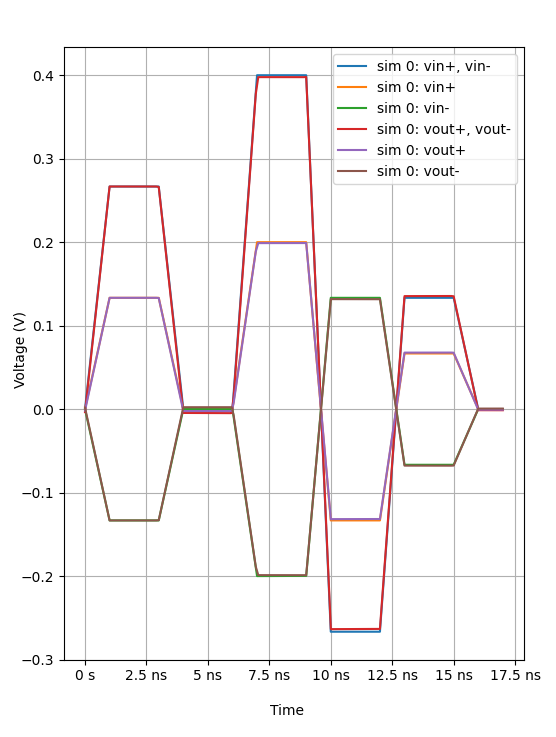
\includegraphics[scale=0.5]{images/wykres.png}
    \caption{Wykres symulacji stworzony przy użyciu Matplotlib}
    \label{fig:wykres_image}
\end{figure}

\subsection{Ćwiczenie dydaktyczne --- modulacje PAM}

W trakcie zajęć laboratoryjnych student będzie miał do dyspozycji symulator phyether, który zawiera implementację wybranych rozwiązań
części standardów 25GBASE-T i 40GBASE-T.

\subsubsection{Wstęp teoretyczny}

Modulacja cyfrowa to technika zamiany bitów na sygnał oraz sygnału na bity. Jest kluczowym zagadnieniem w przesyle danych pomiędzy systemami
komputerowymi. Technologie Ethernetowe wykorzystują wiele technik modulacji. Ćwiczenie te ma na celu przybliżenie oraz porównanie
występujących technik modulacji PAM (Pulse-Amplitude Modulation), która jest jedną z najpopularniejszych w technologii Ethernet.

Najprostszym schematem modulacji jest NRZ --- Non-Return-to-Zero. Chcąc przesłać bit o wartości $0$, na skrętkę zostanie podany sygnał
ujemny, a w przypadku $1$ --- dodatni. Rozwiązanie te niesie za sobą parę wad. Przykładowo, gdy nadawane są długie ciągi zer lub jedynek, sygnał
nie ulega zmianie --- jest to zjawisko niepożądane podczas transmisji i może doprowadzić do desynchronizacji zegarów strony nadawczej i odbiorczej.
Z uwagi na to, NRZ wykorzystywany jest w praktyce w połączeniu z np. kodowaniem liniowym 64b/66b w celu uniknięcia sekwencji zer i jedynek.

PAM jest modulacją, w której dane przesyłane są w postaci zmian amplitudy sygnału. Zmiany te nazywane symbolami. Modulacje PAM różnią się między sobą
liczbą wykorzystywanych poziomów modulacji. PAM3 wykorzystuje trzy poziomy, PAM4 --- cztery, PAM16 --- szesnaście. NRZ można wobec tego nazwać PAM2.
Powodem, dla którego zwiększenie poziomów ma sens jest zwiększona szybkość transmisji. Weźmy na przykład PAM4 --- mając cztery poziomy mamy
do dyspozycji cztery symbole $-3$, $-1$, $1$, $3$, a więc każdy symbol kodować może dwa bity danych. W przypadku NRZ, jeden symbol koduje tylko jeden bit.
Zatem zwiększenie liczby poziomów pozwala na przesył większej ilości bitów przy użyciu jednego symbolu. Schemat ten będzie działał, o ile strona odbiorcza
potrafi rozróżnić poszczególne symbole od siebie, jest to jednak łatwiej osiągalne niż zwiększenie szerokości pasma.
Modulacje PAM4, PAM16 i inne, analogicznie jak NRZ, podatne są na długie ciągi zer i jedynek. Dlatego niezbęde jest zastosowanie różnych `gmatwaczy` bitów, które
zamienią takie sekwencje na bardziej zróżnicowany ciąg np. skrambler.

\subsubsection{Opis narzędzia}

Program phyether, w zakładce `PAM`, posiada symulator modulacji NRZ, PAM4 oraz PAM16, który ilustruje zachowanie sygnału w skrętce podczas transmisji, w zależności
od wybranych modulacji.
Narzędzie będzie wykorzystywane podczas tej części ćwiczenia.

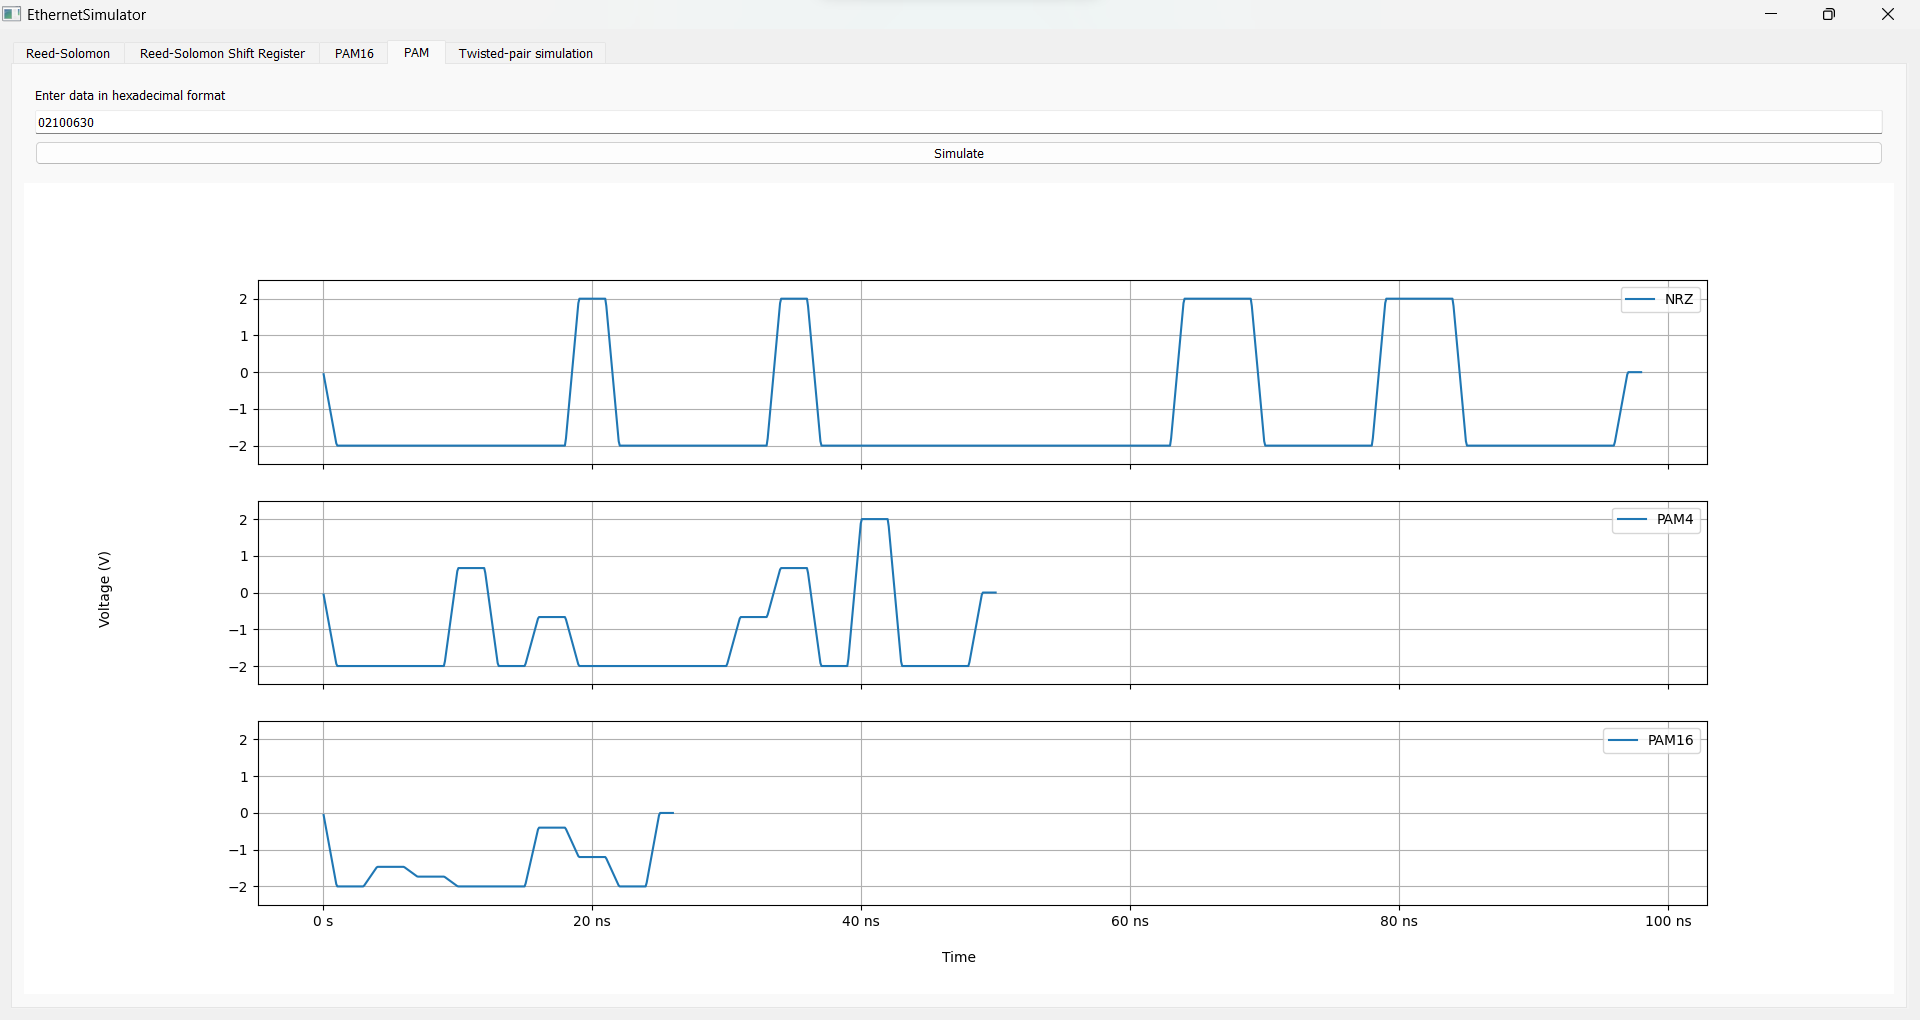
\includegraphics[scale=0.37]{pam_tab.png}

Powyższa grafika prezentuje zakładkę `PAM` programu phyether. Nad przyciskiem \textbf{Simulate} znajduje się pole tekstowe, do którego wpisane mogą być dane w formie
liczb w systemie szesnastkowym. Po wpisaniu danych i kliknięciu \textbf{Simulate}, wpisane dane zamieniane są na symbole modulacji NRZ, PAM4 oraz PAM16, które
następnie wysyłane są na medium. Wynik symulacji przedstawiony jest w dolnej części zakładki.

\subsubsection{Zadania do realizacji}

\begin{enumerate}
    \item Zamień numer swojego indeksu na postać szesnastkową i wykorzystaj go jako liczbę do przesłania. Przeprowadź symulację. Zanotuj w sprawozdaniu
    przybliżony czas transmisji oraz liczbę poziomów natężenia. Opisz wnioski, które nasuwają Ci się po wykonanym ćwiczeniu.
    \item Prześlij ciąg składający się z samych jedynek (fffffff \dots) lub samych zer (000000 \dots). Popatrz na wynik symulacji. Jak nazywa się zaobserwowane zjawisko? Czy znasz sposoby,
    które zapobiegają jego wystąpieniu? Zanotuj w sprawozdaniu.
\end{enumerate}

\subsection{Ćwiczenie dydaktyczne --- PAM16 w 40GBASE-T}
\subsubsection{Wstęp teoretyczny}
Ciekawą kwestią w przypadku modulacji PAM jest także zamiana bitów na konkretne symbole alfabetu modulacji.
Możemy sobie wyobrazić, że w najprostszym przypadku wartość 0 mapowana jest na najmniejszy symbol, natomiast 1111
--- na największy. Istnieją także bardziej wyrafinowane sposoby mapowania, przykładowo popularnym jest zastosowanie kodu Graya.
W tym ćwiczeniu zobaczymy podejście, które zostało zastosowane w standardach 25GBASE-T oraz 40GBASE-T.

Wyżej wymienione standardy korzystają z modulacji PAM16, natomiast symbole nadawane na parach skrętki wybierane są według diagramu
konstelacji DSQ128. Aby wyjaśnić czym on jest, spójrzmy pierw na 64QAM (Quadrature Amplitude Modulation). 64QAM to modulacja, która jest
połączeniem modulacji amplitudy oraz fazy (dane kodowane są poprzez zmianę amplitudy oraz fazy sygnału). Symbole wybierane są na podstawie
diagramu konstelacji 64QAM --- rys.~\ref{fig:lab-64QAM}.

Diagram podzielony jest na cztery części. Oś X odnosi się do fazy, a oś Y --- amplitudy. Każdy symbol, który chcemy nadać,
jest krotką (x, y), która oznacza punkt na diagramie dla danej wartości. Jak można zauwarzyć, sąsiednie punkty różnią się
między sobą jednym bitem --- dzięki czemu, gdy nastąpi przekłamanie, najprawdopodobniej tylko jeden bit będzie zły.

W standardach 25GBASE-T i 40GBASE-T symbole dobierane są na podstawie diagramu konstelacji DSQ128, który jest złożeniem dwóch
diagramów 64QAM - rys. \ref{fig:lab-dsq128}.

Dane grupowane są w 7-bitowe grupy ($u_0$, $u_1$, $u_2$), ($c_0$, $c_1$, $c_2$, $c_3$), po czym każda taka grupa mapowana jest na krotkę (PAM16$_1$, PAM16$_2$) według algorytmu:

Krok 1:
\begin{align*}
    x_{13} &= \neg u_0 * u_2 \\
    x_{12} &= u_0 \oplus u_2 \\
    x_{11} &= c_0 \\
    x_{10} &= c_0 \oplus c_1 \\
    x_{23} &= (u_1 * u_2) + (u_0 * \neg u_1) \\
    x_{22} &= u_1 \oplus u_2 \\
    x_{21} &= c_2 \\
    x_{20} &= c_2 \oplus c_3
\end{align*}

Krok 2:
\begin{align*}
    x_1 &= 8x_{13} + 4x_{12} + 2x_{11} + x_{10} \\
    x_2 &= 8x_{23} + 4x_{22} + 2x_{21} + x_{20}
\end{align*}

Krok 3:
\begin{align*}
    y_1 &= (x_1 + x_2) \mod 16 \\
    y_2 &= (-x_1 + x_2) \mod 16
\end{align*}

Krok 4:
\begin{align*}
    \text{PAM16}_1 &= 2y_1 - 15 \\
    \text{PAM16}_2 &= 2y_2 - 15
\end{align*}

Symbole są następnie nadawane na kolejnych parach skrętki:
\begin{table}[h]
    \centering
    \resizebox{\textwidth}{!}{%
    \begin{tabular}{c | c c c c c c c |}
        \cmidrule{2-8}
        Pair A & PAM16$_1$<0> & PAM16$_2$<0> & PAM16$_1$<4> & PAM16$_2$<4> & \ldots & PAM16$_1$<508> & PAM16$_2$<508> \\
        \cmidrule{2-8}
        Pair B & PAM16$_1$<1> & PAM16$_2$<1> & PAM16$_1$<5> & PAM16$_2$<5> & \ldots & PAM16$_1$<509> & PAM16$_2$<509> \\
        \cmidrule{2-8}
        Pair C & PAM16$_1$<2> & PAM16$_2$<2> & PAM16$_1$<6> & PAM16$_2$<6> & \ldots & PAM16$_1$<510> & PAM16$_2$<510> \\
        \cmidrule{2-8}
        Pair D & PAM16$_1$<3> & PAM16$_2$<3> & PAM16$_1$<7> & PAM16$_2$<7> & \ldots & PAM16$_1$<511> & PAM16$_2$<511> \\
        \cmidrule{2-8}
    \end{tabular}}
\end{table}

\begin{figure}[h]
    \centering
    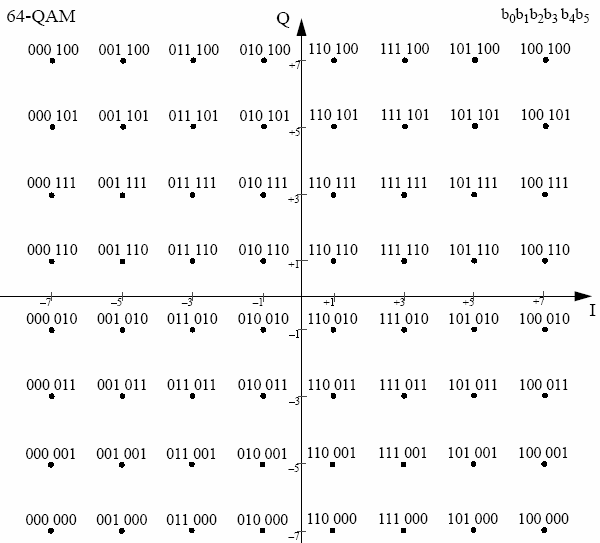
\includegraphics[scale=0.4]{64QAM-constellation-diagram.png}
    \caption{Diagram konstelacji 64QAM}
    \label{fig:lab-64QAM}
\end{figure}

\begin{figure}[h]
    \centering
    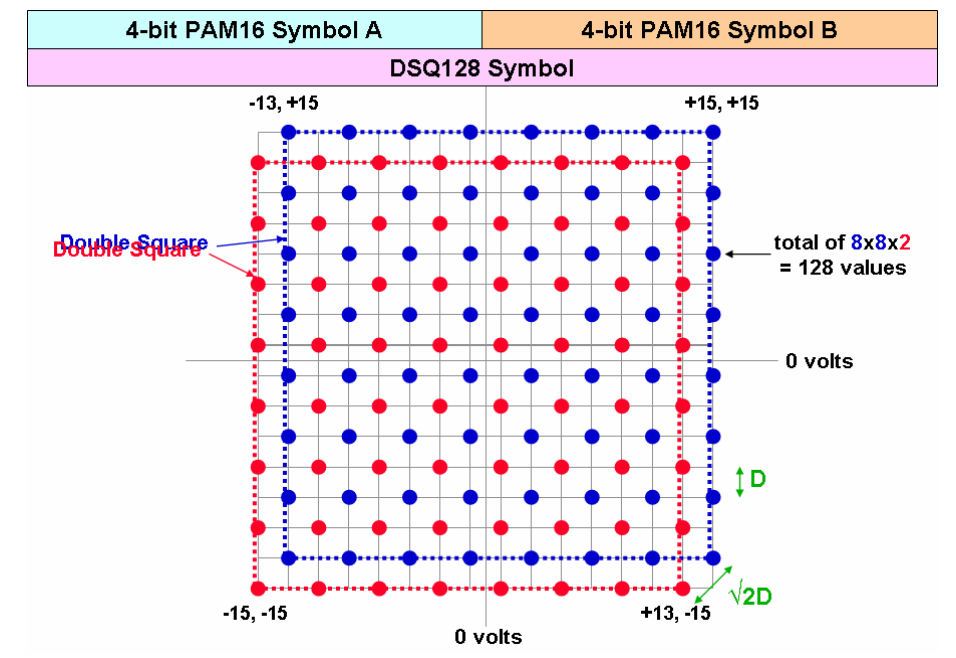
\includegraphics[scale=0.4]{dsq128.png}
    \caption{Diagram konstelacji DSQ128}
    \label{fig:lab-dsq128}
\end{figure}

\clearpage

\subsubsection{Zadania do realizacji}

\begin{enumerate}
    \item Zastosowanie DSQ128 nie eliminuje możliwości wystąpienia stałej składowej. Znajdź ciąg, który
    temu dowodzi i zanotuj go w sprawozdaniu.
\end{enumerate}
